\documentclass[11pt, a4paper]{report}

\usepackage[T1]{fontenc}
\usepackage[utf8]{inputenc}
\usepackage[ngerman]{babel}
\usepackage{graphicx}
\usepackage{wrapfig}
\usepackage{listings}
\usepackage{amsmath}
\allowdisplaybreaks
\usepackage{mathtools}
\usepackage{amsfonts}
\usepackage{amssymb}
\usepackage{thmtools}
\usepackage[center]{caption}
\setlength{\parindent}{0pt}
\usepackage{grffile}

\usepackage[ 
  style=alphabetic, 
  sorting=nty, 
  sortcites=true, 
  autopunct=true, 
  babel=hyphen, 
  hyperref=true, 
  abbreviate=false, 
  backref=true, 
  backend=bibtex, 
  block=space
  ] { biblatex }

\usepackage{fancyhdr}
\fancypagestyle{plain}{
  \fancyhf{}
  \fancyfoot[R]{\thepage}
  \renewcommand{\headrulewidth}{0pt}
  \renewcommand{\footrulewidth}{0pt}
}

\makeatletter
  \newcommand\flausr{\@fleqntrue} %align linksbündig
\makeatother

\makeatletter
\renewcommand\@dotsep{2}
\makeatother

\newcommand{\lnn}[1]{%
  \ln\left(#1\right)%
}

\graphicspath{}

\addbibresource{bib.bib}
\defbibheading{bibempty}{}

\usepackage[pdfborder={0 0 0}]{hyperref}

\usepackage{breakurl}


\begin{document}

\title{ \underline{Eine Einführung in die Differentialrechnung}}
\author{Studienarbeit\\
  \\
  Name des Studiengangs:\\
  \Large Life Science Engineering\\  
  \Large \textbf{Fachbereich 2}  
  \\
  \\  
  vorgelegt von:\\
  \Large Hendrik Schroeder\\
  s0564364@htw-berlin.de\\
  \\ 
  \\
  \\
  \Large Wissenschaftliches Arbeiten mit \LaTeX{}\\
  Hochschule für Technik und Wirtschaft\\
  \\
  Berlin
  \\
  \\
  Moin\\
  \\
  Gutachter: Marcel 
  \\
  \\
  \\
  \\}
  \date{Datum:\\
  08. Februar, 2020}
\maketitle

\setcounter{tocdepth}{2}
\tableofcontents
\clearpage

\listoffigures
\addcontentsline{toc}{chapter}{Abbildungsverzeichnis}
\clearpage

\listoftables
\addcontentsline{toc}{chapter}{Tabellenverzeichnis}
\clearpage

\chapter{Ableitungsbegriff}
Die Differentialrechnung ist ein Gebiet der Mathematik, welches zusammen mit der Integralrechnung dem Begriff der Infinitesimalrechnung untergeordnet wird und somit zur Analysis gehört. Die Differentialrechnung ist im Wesentlichen auf die beiden Mathematiker Isaac Newton und Gottfried Wilhelm Freiherr von Leibniz zurückzuführen \cite[Seite 188]{Wendland.2005}. Die durch Newton und Leibniz definierte lokale Änderungsrate, auch Ableitung oder momentane Änderungsrate genannt steht dabei im Mittelpunkt der Differentialrechnung.


\section{Differenzenquotient}
Der Begriff der Ableitung basiert auf dem Anstieg der Tangente  an einem Punkt $P(x_0,f(x_0))$ \cite[Seite 141]{Stewart.2015}.
\\
\begin{wrapfigure}{o}{6 cm}
\centering
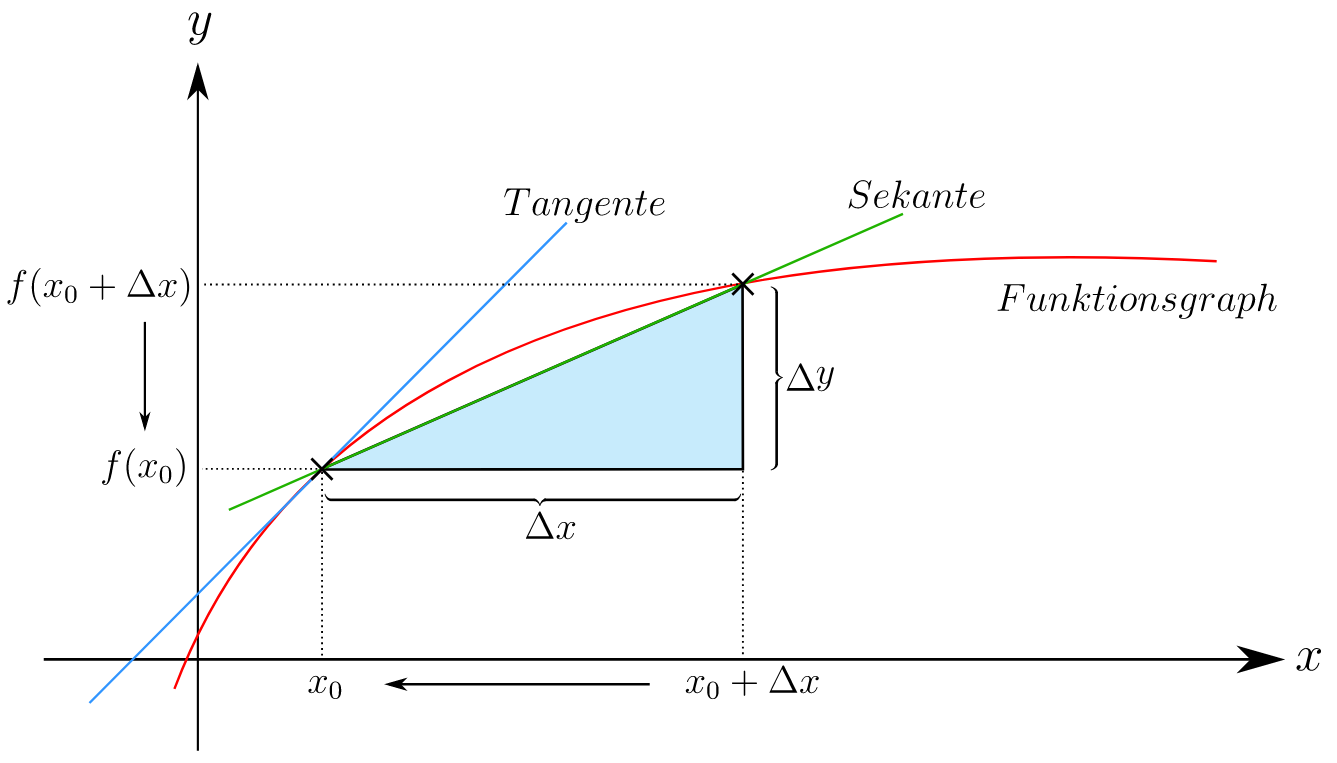
\includegraphics[scale=0.25]{fig/Ableitung}
\caption[Approximation der Tangente durch Verringerung von $\Delta x$]{Approximation der Tangente durch Verringerung von $\Delta x$ \cite{JohannesSchneider.2015}}
\label{fig:Ableitung}
\end{wrapfigure} 
Bei einer beliebigen Funktion $f:D \rightarrow \mathbb{R}$ mit der Gleichung $y = f(x)$ und $x \in D \setminus \lbrace x_0 \rbrace$ lässt sich die mittlere Änderungsrate, also der Anstieg in einem Intervall $I = \lbrack x_0,x_0+\Delta x \rbrack$ über den Quotienten 
\begin{align}
\frac{\Delta y}{\Delta x}:&=\frac{f(x_0+\Delta x)-f(x_0)}{(x_0+\Delta x)-x_0}\\
&= \frac{f(x_0+\Delta x)-f(x_0)}{\Delta x}\label{DefDifferenzenquo}\\
&= \frac{f(x)-f(x_0)}{x-x_0}
\end{align}
berechnen.
\clearpage
Um nun den Anstieg der Tangente am Punkt $P(x_0,f(x_0))$ ermitteln zu können und nicht den Anstieg einer Sekante durch die Punkte $P(x_0,f(x_0))$ und $Q(x_0+\Delta x,f(x_0+\Delta x))$ der Funktion muss $\Delta x$ oder gegen Null gehen oder anders gesagt $x$ gegen $x_0$ gehen (siehe Abb.~\ref{fig:Ableitung}). 


\section{Grenzwerte und Differentialquotient}
Das Annähern einer Funktion an einen bestimmten Wert in der Umgebung der Stelle wird als Grenzwert bezeichnet. Wenn c eine Konstante ist und die beiden Grenzwerte $\lim\limits_{x \to a}{f(x)}$ und $\lim\limits_{x \to a}{g(x)}$ existieren, gelten folgende Grenzwertsätze \cite[Seite 141 ff.]{Stewart.2015}:
\begin{center}
\captionof{table}{Auflistung wichtiger Grenzwertsätze}
\begin{tabular}[h]{|c|p{9cm}|}
\hline
\multicolumn{1}{|c}{Name} & \multicolumn{1}{|c|}{Grenzwertsatz}\\ \hline %kein schöner Stil, aber klappt
	Summenregel & $\lim\limits_{x \to a}{\lbrack f(x)+g(x)\rbrack} = \lim\limits_{x \to a}{f(x)}+\lim\limits_{x \to a}{g(x)}$\\ \hline
	Differenzenregel & $\lim\limits_{x \to a}{\lbrack f(x)-g(x)\rbrack} = \lim\limits_{x \to a}{f(x)}-\lim\limits_{x \to a}{g(x)}$\\ \hline
	Konstantenregel & $\lim\limits_{x \to a}{\lbrack c \cdot f(x) \rbrack} = c \cdot \lim\limits_{x \to a}{f(x)}$\\ \hline
	Produktregel & $\lim\limits_{x \to a}{\lbrack f(x) \cdot g(x)\rbrack} = \lim\limits_{x \to a}{f(x)} \cdot \lim\limits_{x \to a}{g(x)}$\\ \hline
	Quotientenregel & $\lim\limits_{x \to a}{\dfrac{f(x)}{g(x)}} = \dfrac{\lim\limits_{x \to a}{f(x)}}{\lim\limits_{x \to a}{g(x)}}$ für $\lim\limits_{x \to a}{g(x)}\neq 0$\\ \hline
	Schachtelungssatz & wenn $|f(x)|\le |g(x)|$ und $\lim\limits_{x \to a}{g(x)} = 0$, dann ist $\lim\limits_{x \to a}{f(x)} = 0$\\ \hline
	Kettenregel & wenn $g(b)$ stetig ist, $\lim\limits_{x \to a}{f(x)} = b$ und $\lim\limits_{z \to b}{f(z)} = c$ mit $b,c \in \mathbb{R}$, dann gilt $\lim\limits_{x \to a}{g(f(x))} = c$ \\ \hline
\end{tabular}
\label{tab:Grenzwertsätze}
\end{center}

Die in Tabelle ~\ref{tab:Grenzwertsätze} aufgelisteten Grenzwertsätze sind lediglich die Wichtigen. Aus diesen folgen weitere Regeln. So ergibt sich beispielsweise aus der Produktregel und der Annahme $f(x) = g(x)$ für $n \in \mathbb{N}^{+}$ 
\begin{equation}
\lim\limits_{x \to a} {\lbrack (x) \rbrack^{n}} = \lbrack \lim\limits_{x \to a} { (x) \rbrack^{n}} 
\end{equation}
die Potenzregel.
\\
Der Begriff des Grenzwerts lässt sich nun auf den Differenzenquotient
\begin{equation}
f^{\prime}(x):= \lim\limits_{x \to x_0}{\dfrac{f(x)-f(x_0)}{x-x_0}} := \dfrac{df}{dx}
\end{equation}
übertragen. Da die Differenzen nun infinitesimal kleine Größen annehmen, die sogenannten Differentiale, wird der Ausdruck Differentialquotient $\dfrac{df}{dx}$ eingeführt. Dieser beschreibt die momentane Änderungsrate im Punkt $P(x_0,f(x_0))$. Geometrisch gesehen beschreibt dies gerade den Anstieg der Tangente in dem Punkt $P(x_0,f(x_0))$ \cite[Seite 183]{FRITZSCHE.2020}. Falls dieser Differentialquotient existiert wird eine Funktion differenzierbar in $x_0$ genannt \cite[Seite 189]{Wendland.2005}.
Oft wird die Differenzierbarkeit einer Funktion an einer bestimmten Stelle auch über die Existenz eines Anstiegs einer Sekante
\begin{equation}
m_S = \frac{f(x_0+h)-f(x_0)}{h}
\end{equation}
durch die beiden Punkte $P(x_0,f(x_0))$ und $Q(x_0+h,f(x_0+h))$ definiert, wobei $h \in \mathbb{R}$ ist und $x_0+h$ im Intervall $I = \lbrack x_0,x \rbrack$ liegt.
Die daraus resultierende Sekantengleichung \cite[Seite 99 f.]{Deitmar.2017}
\begin{equation}
S_h(x) = f(x_0)+m_S \cdot (x-x_0)
\end{equation}
approximiert die Tangente \cite[192]{Wendland.2005}
\begin{equation}
T(x) = f(x_0)+m \cdot (x-x_0)
\end{equation}
am Punkt $P(x_0,f(x_0))$, wenn der Anstieg bei h gegen Null konvergiert \cite[184]{FRITZSCHE.2020}.


\chapter{Berechnungen}


\section{Ableitungsfunktion über Differenzenquotient}
Die obige Definition einer Ableitung ist  abhängig von einem bestimmten Punkt, in dem Fall $P(x_0, f(x_0))$. Der Begriff der Ableitungsfunktion $f^{\prime}(x)$ erweitert dies und beschreibt die Funktion, welche sich aus der Gesamtheit der Ableitungen des Definitionsbereichs $D$ von $f$ ergibt \cite[Seite 19]{Borgwadt.1994}.
\begin{equation}
f^{\prime}:x \rightarrow f^{\prime}(x), x \in D
\end{equation}
Der Definitionsbereich $\Omega$ von $f^{\prime}(x)$ ist daher gleichbedeutend mit den Stellen, an denen die Funktion differenzierbar ist. Die Ableitungsfunktion ist geometrisch betrachtet die Funktion, welche allen differenzierbaren Stellen aus dem Definitionsbereich der Funktion die Anstiege dieser zuordnet. 
Die ursprüngliche Berechnung der Ableitungsfunktion folgt also über die Definition des Differenzenquotienten (siehe Formel ~\ref{DefDifferenzenquo}), wobei sich $\Delta x$ dem Wert Null annähert.


\section*{Beispiele}
\begin{enumerate}
\item Ableitung von $f(x) = x$:
\begin{align*}
\dfrac{\Delta x}{\Delta y} &= \dfrac{f(x_0+\Delta x)-f(x_0)}{\Delta x}\\
&=\dfrac{(x_0+\Delta x)-(x_0)}{\Delta x}\\
&=\dfrac{x_0-x_0+\Delta x}{\Delta x}\\
&=\dfrac{\Delta x}{\Delta x} = 1
\end{align*}
\clearpage

\item Ableitung von $f(x) = x^2+5x-9$:
\begin{align*}
\dfrac{\Delta x}{\Delta y} &= \dfrac{f(x_0+\Delta x)-f(x_0)}{\Delta x}\\
&=\dfrac{((x_0+\Delta x)^{2}+5\cdot(x_0+\Delta x)-9)-(x_0^{2}+5\cdot x_0-9)}{\Delta x}\\
&=\dfrac{x_0^{2}+2\cdot x_0 \cdot \Delta x+\Delta x^{2}+5\cdot x_0+5\cdot \Delta x-9-x_0^{2}-5\cdot x_0+9}{\Delta x}\\
&=\dfrac{2\cdot x_0\cdot \Delta x + \Delta x^{2}+5\cdot \Delta x}{\Delta x}\\
&=2\cdot x_0+\Delta x+5
\end{align*} % es wurde \Delta x^{2} und nicht (\Delta x)^{2} geschrieben -> sah meiner Meinung nach besser aus

Somit ergibt sich folgende Ableitungsfunktion:
\begin{equation}
f^{\prime}(x_0)= \lim\limits_{\Delta x \to 0}{2\cdot x_0+\Delta x+5} = 2\cdot x_0+5
\end{equation}

\begin{center}
\begin{figure}[h]
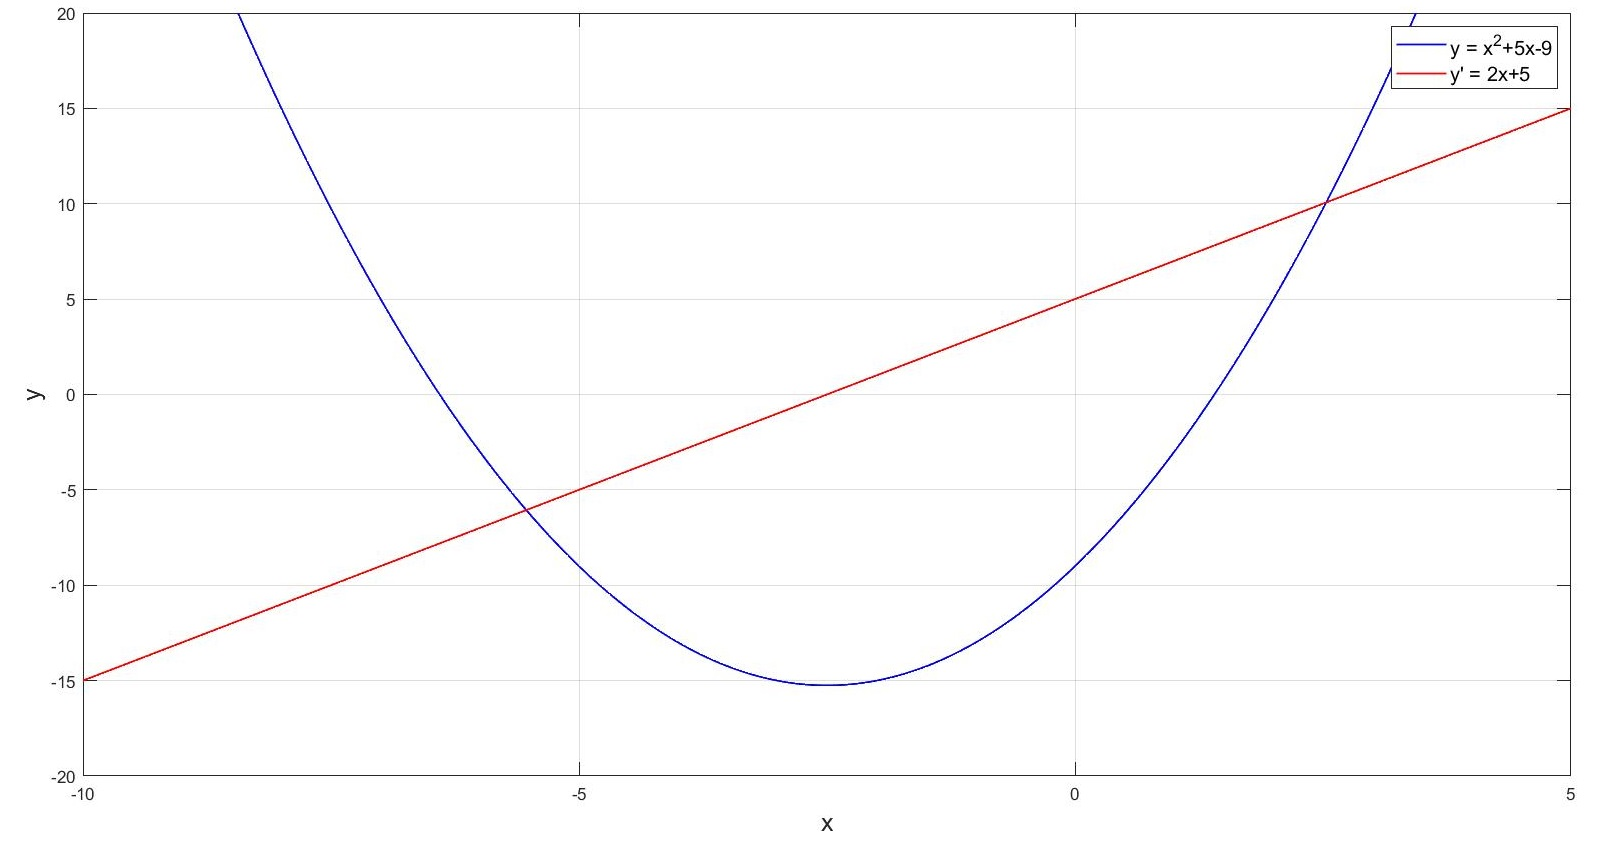
\includegraphics[scale=0.3]{fig/Ableitung_Differenzenquotient_Nr2}
\caption[Funktion $f(x) = x^2+5x-9$ und ihre Ableitungsfunktion]{Funktion $f(x) = x^2+5x-9$ und ihre Ableitungsfunktion $f^{\prime}(x)= 2\cdot x+5$}
\label{fig:AbleitungDifferenzenquo1}
\end{figure}
\end{center}

\item Ableitung von $f(x)= \ln{x}$ unter der Nutzung der  Substitution $n=\dfrac{\Delta x}{x_0}$, woraus $\Delta x = n \cdot x_0$ und $\dfrac{1}{\Delta x}= \dfrac{1}{n} \cdot \dfrac{1}{x_0}$ folgt:
\begin{align*}
\dfrac{\Delta x}{\Delta y} &= \dfrac{f(x_0+\Delta x)-f(x_0)}{\Delta x}\\
\displaybreak
&= \dfrac{\lnn{x_0+\Delta x}-\lnn{x_0}}{\Delta x}\\
&= \dfrac{\lnn{\dfrac{x_0+\Delta x}{x_0}}}{\Delta x}\\
&= \dfrac{1}{\Delta x} \cdot \lnn{1+\dfrac{\Delta x}{x_0}}\\
&= \lnn{(1+\dfrac{\Delta x}{x_0})^{\dfrac{1}{\Delta x}}}\\
&= \lnn{(1+n)^{\dfrac{1}{n} \cdot \dfrac{1}{x_0}}}\\
&= \lnn{((1+n)^{\dfrac{1}{n}})^\frac{1}{x_0}}\\
&= \dfrac{1}{x_0} \cdot \lnn{(1+n)^{\frac{1}{n}}}
\end{align*}

Somit ergibt sich folgende Ableitungsfunktion:
\begin{align*}
f^{ \prime} (x_0) &= \dfrac{1}{x_0} \cdot \lnn{\lim\limits_{\Delta x \to 0}{(1+n)^{\dfrac{1}{n}}}} \\
&= \dfrac{1}{x_0} \cdot \lnn{e} = \frac{1}{x_0}
\end{align*}

\begin{center}
\begin{figure}[h]
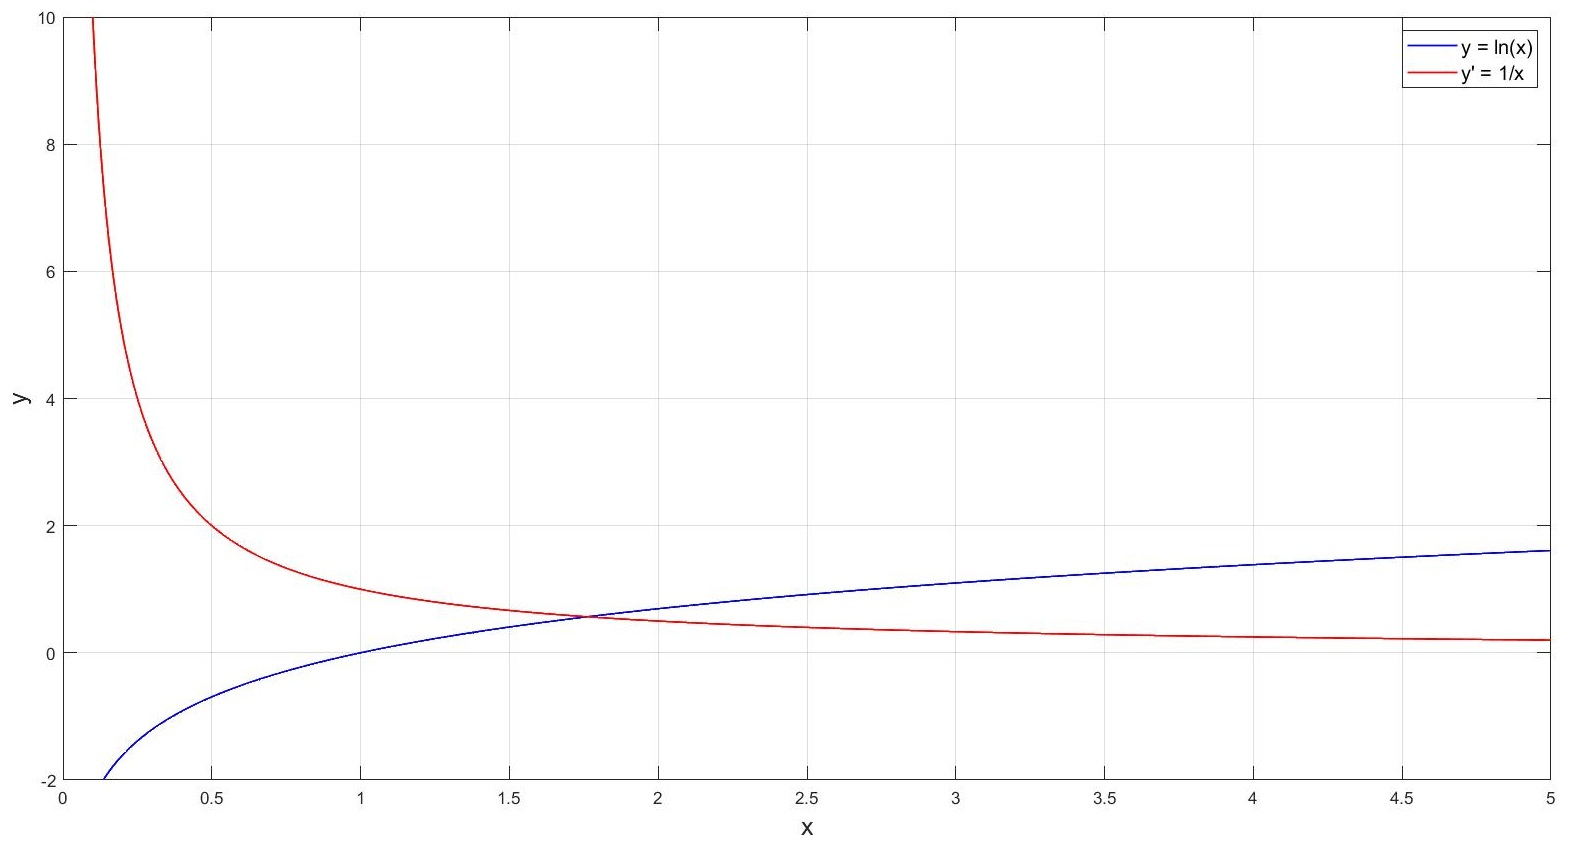
\includegraphics[scale=0.3]{fig/natural_log_and_prime}
\caption[Funktion $f(x) = \lnn{x}$ und ihre Ableitungsfunktion]{Funktion $f(x) = \lnn{x}$ und ihre Ableitungsfunktion $f^{\prime}(x)= \frac{1}{x}$}
\label{fig:AbleitungDifferenzenquo2}
\end{figure}
\end{center}
\end{enumerate}


\section{Ableitungsregeln}
Aus der ursprünglichen Methode der Berechnung von Ableitungsfunktionen und den Grenzwertsätzen ergeben sich für die differenzierbaren Funktionen $f(x)$ und $g(x)$ folgende Ableitungsregeln \cite[Seite 192]{Wendland.2005}

\begin{center}
\captionof{table}{Auflistung wichtiger Ableitungsregeln}
\begin{tabular}[h]{|c|p{9cm}|}
\hline
\multicolumn{1}{|c}{Name} & \multicolumn{1}{|c|}{Ableitungsregel}\\ \hline %kein schöner Stil, aber klappt
	Konstante Funktion & $\lbrack a \rbrack^{\prime}=0$ für $\alpha \in \mathbb{R}$\\ \hline
	Faktorregel & $\lbrack \alpha \cdot f(x) \rbrack^{\prime} = \alpha \cdot f^{\prime}(x)$\\ \hline
	Linearität & $\lbrack f(x) \pm g(x) \rbrack^{\prime}= f^{\prime}(x) \pm g^{\prime}(x)$\\ \hline
	Produktregel & $\lbrack f(x) \cdot g(x) \rbrack^{\prime}= f^{\prime}(x) \cdot g(x) + f(x) \cdot g^{\prime}(x)$\\ \hline
	Quotientenregel & 
\setlength\abovedisplayskip{-10pt} % Abstand über Gleichung bei alignat verringern
\setlength\belowdisplayskip{-6pt} % Abstand unter Gleichung bei align verringern
\begingroup %align linksbündig
  \flausr {\begin{alignat*}{2}
	\left[ \dfrac{f(x)}{g(x)} \right]^{\prime} &=  \dfrac{f^{\prime}(x)}{g(x)}- \dfrac{f(x)}{g^{2}(x)} \cdot g^{\prime}(x) \\
	&= \dfrac{f^{\prime}(x)\cdot g(x)-f(x) \cdot g^{\prime}(x)}{g^{2}(x)}
	\end{alignat*}} \endgroup \\ \hline
	Kettenregel & $[f \circ g]^{\prime}(x) = [f(g(x))]^{\prime}=f^{\prime}(g(x)) \cdot g^{\prime}(x)$ \\ \hline
\end{tabular}
\label{tab:Ableitungsregeln}
\end{center}

Weitere Regeln, wie beispielsweise die Reziprokenregel
\begin{equation*}
\left[ \frac{1}{f(x)} \right]^{\prime} = \frac{f(x) \cdot 0-f^{\prime}(x) \cdot 1}{f^{2}(x)}= \frac{-f^{\prime}(x)}{f^{2}(x)}
\end{equation*}
ergeben sich direkt aus den in Tabelle ~\ref{tab:Ableitungsregeln} aufgelisteten Ableitungsregeln. 


\section*{Beispiele} % nicht im Inhaltsverzeichnis aufgelistet
\begin{enumerate}
	\item Konstante Funktion:
		\begin{align*}
		\left[ 5 \right]^{\prime} = 0
		\end{align*}	 
	\item Faktorregel 
		\begin{enumerate}
			\item Erste Ableitung:
				\begin{align*}
				\left[ 8\cdot x^{2} \right]^{\prime} &= 8\cdot \left[ x^{2} \right]^{\prime}\\
				&= 8 \cdot 2 \cdot x \\
				&= 16 \cdot x
				\end{align*}
			\item Zweite Ableitung:\\
				Auch die Ableitungsfunktion kann, sofern sie differenzierbar ist, abgeleitet werden. Höhere Ableitungen werden mit ihrer 						Ordnung assoziiert. Es haben sich für die Ordnung $2$ die Bezeichnungen 
				\begin{equation}
				f^{\prime\prime}(x)= f^{(2)}(x) =\dfrac{d^{2}f(x)}{dx^{2}} := f^{\prime}\lbrack f^{\prime}(x)\rbrack 
				\end{equation}
				eingebürgert.
				\begin{align*}
				\left[ 8\cdot x^{2} \right]^{\prime\prime} &= \left[ 16 \cdot x \right]^{\prime}\\
				&= 16 \cdot \left[ x \right]^{\prime}\\
				&= 16 \cdot 1 \\
				&= 16
				\end{align*}
		\end{enumerate}
	\item Summenregel:
		\begin{enumerate}
			\item Erste Ableitung:
				\begin{align*}
				\left[ x^{5} + 2 \cdot x \right]^{\prime} &= \left[ x^{5} \right]^{\prime} + \left[ 2\cdot x \right]^{\prime} \\
				&= \left[ x^{5} \right]^{\prime} + 2\cdot \left[ x \right]^{\prime}\\
				&= 5\cdot x^{4} + 2
				\end{align*}
			\item Zweite Ableitung:
				\begin{align*}
				\left[ x^{5} + 2 \cdot x \right]^{\prime\prime} &= \left[ 5\cdot x^{4} + 2 \right]^{\prime} \\
				&= \left[ 5\cdot x^{4} \right]^{\prime} + \left[ 2 \right]^{\prime} \\
				&= 5\cdot \left[ x^{4} \right]^{\prime} + \left[ 2 \right]^{\prime} \\
				&= 5\cdot 4 \cdot x^{3} + 0 \\
				&= 20 \cdot x^{3}
				\end{align*}
		\end{enumerate}
	\item Produktregel:
		\begin{enumerate}
			\item Erste Ableitung:
				\begin{align*}
				\left[ x^{2} \cdot \sin (x) \right]^{\prime} \\ 
				&= \left[ x^{2} \right]^{\prime} \cdot \sin (x) + x^{2} \cdot \left[ \sin (x) \right]^{\prime} \\
				&= 2x \cdot \sin (x) + x^{2} \cdot \cos (x) 
				\end{align*}
			\item Zweite Ableitung:
				\begin{align*}
				\left[ x^{2} \cdot \sin (x) \right]^{\prime\prime} &= \left[ 2x \cdot \sin (x) + x^{2} \cdot \cos (x) \right]^{\prime} \\
				&= 2 \cdot \sin (x) + 2x \cdot \cos (x) + 2x \cdot \cos (x) + x^{2} \cdot -\sin (x)\\
				&= 2 \cdot \sin (x) + 4x \cdot \cos (x) - x^{2} \cdot \sin (x)
				\end{align*}
		\end{enumerate}
	\item Quotientenregel:
		\begin{enumerate}
			\item Erste Ableitung:
				\begin{align*}
				\left[ \dfrac{1+x}{4x} \right]^{\prime} &=  \dfrac{4x \cdot 1 - ((1+x)\cdot 4)}{16x^{2}}\\
				&= \dfrac{4x - 4 -4x}{16x^{2}}\\
				&= \dfrac{-4}{16x^{2}}\\
				&= \dfrac{-1}{4x^{2}}
				\end{align*}
			\item Zweite Ableitung:
				\begin{align*}
				\left[ \dfrac{1+x}{4x} \right]^{\prime\prime} &= \left[ \dfrac{-1}{4x^{2}} \right]^{\prime}\\
				&= \dfrac{4x \cdot 0 - (-1 \cdot 2 \cdot 4x)}{16x^{4}}\\
				&= \dfrac{8x}{16x^{4}}\\
				&= \dfrac{1}{2x^{3}}
				\end{align*}
		\end{enumerate}
	\item Kettenregel:
		\begin{enumerate}
			\item Erste Ableitung:
				\begin{align*}
				\left[ (x^{5}+6)^{4} \right]^{\prime} &= 4 \cdot (x^{5}+6)^{3} \cdot (5x^{4}+0) \\
				&= 20x^{4} \cdot (x^{5}+6)^{3}
				\end{align*}
			\item Zweite Ableitung:
				\begin{align*}
				\left[ (x^{5}+6)^{4} \right]^{\prime\prime} &= \left[ 20x^{4} \cdot (x^{5}+6)^{3} \right]^{\prime} \\
				&= 80x^{3} \cdot (6+x^{5})^{3}+20x^{4} \cdot 3 \cdot (6+x^{5})^{2} \cdot 5x^{4}\\
				&= 80x^{3} \cdot (6+x^{5})^{3} + 300x^{8} \cdot (6+x^{5})^{2}
				\end{align*}
		\end{enumerate}
\end{enumerate}
\clearpage


\chapter{Hauptsätze und weitere Themen der Differentialrechnung}
\section*{Fundamentalsatz der Analysis}
Der Fundamentalsatz der Analysis besteht aus zwei Teilen, welche die Antiableitung, auch Stammfunktion genannt, beschreiben.
\begin{enumerate}
\item Erster Teil \cite[Seite 392]{Stewart.2015}
Wenn eine Funktion $f(x)$ im Intervall $P \subset \mathbb{R}$ stetig ist, so ist die Funktion 
\begin{equation}
G(x)=\int_{a}^{x}f(t)dt
\end{equation}
unter der Voraussetzung, dass $a \in P$ ist, stetig differenzierbar und die sogenannte Stammfunktion von $f(x)$. Dies bedeutet, dass unabhängig von $a$ die Ableitung $G^{\prime}(x)= f(x)$ ist. Der Vorgang der Stammfunktionsbestimmung wird unter dem Begriff Integration aufgefasst.
\item Zweiter Teil \cite[396]{Stewart.2015}
Wenn eine Funktion f(x) stetig im Intervall $\left[ a,b \right]$ mit $a,b \in \mathbb{R}$ ist, dann gilt 
\begin{equation}
\int_{a}^{b}f(x)dx=G(b)-G(a)
\end{equation}
für die Stammfunktion G(x).
\end{enumerate}

\section*{Mittelwertsatz der Differentialrechnung}
Der Mittelwertsatz der Differentialrechnung besagt, dass eine im Intervall $\left[ a,b \right]$ mit $a<b$ und $a,b \in \mathbb{R}$ stetige und differenzierbare Funktion $f(x)$ mindestens für  einen Wert $\Lambda$ definiert ist, welche folgende Eigenschaft aufweist \cite[Seite 106]{Deitmar.2017}
\begin{equation}
f^{\prime}(\Lambda)= \dfrac{f(b)-f(a)}{b-a}
\end{equation}
Einfach gesagt gibt es also immer mindestens einen Punkt in dem Intervall $\left[ a,b \right]$, welcher die gleiche Steigung, wie eine Sekante durch die Punkte $P(a,f(a))$ und $Q(b,f(b))$ aufweist.


\section*{Weiterführende Themen der Differentialrechnung}
Da eine Einführung nur einen marginalen Anteil an Grundlagen der Differentialrechnung abdecken kann, werden als Ausblick ein paar weiterführende Themen und Bereiche, welche Ableitungen nutzen, benannt.\\ 
\begin{itemize}
	\item Taylorreihen
	\item gewöhnliche Differentialgleichungen
	\item Differentialrechnung von komplexen Funktionen
	\item Differentialrechnung von Funktionen mehrerer Veränderlichen
	\item partielle Differentialgleichungen
	\item Differentialgeometrie
\end{itemize}

Ableitungen werden nahezu universell in der Mathematik und der Physik verwendet. Auch in Bereichen der Mathematik, in welchen die Nutzung von Ableitungen auf den ersten Blick für nicht relevant erscheint, wie beispielsweise die Maßtheorie, basieren bedeutende Theoreme und Definitionen auf dem Prinzip  der Ableitung.
\newpage


\chapter*{Literatur}
\addcontentsline{toc}{chapter}{Literaturverzeichnis}

\nocite{Borgwadt.1994}		% Differentialrechnung
\nocite{Deitmar.2017}		% Analysis
\nocite{FRITZSCHE.2020}		% GRUNDKURS ANALYSIS: Differentiation und integration in einer vernderlichen			
\nocite{Stewart.2015}		% Calculus, Early Transcendentals, International Metric Edition
\nocite{Wendland.2005}		% Analysis: Integral- und Differentialrechnung, gew{\"o}hnliche Differentialgleichungen, komplexe Funktionentheorie
\nocite{Wikipedia.23.01.2020} % Differentialrechnung
\printbibliography[
	heading=subbibintoc,
	type=book,
	title={Bücher}
	]
\printbibliography[
	heading=subbibintoc,
	type=misc,
	title={Internetquellen}
	]
\end{document}
